%!TEX root = ../../../main.tex


\section[Antennas]{Coupling \Nds to Double Bowtie Antenna Structures} \label{sec::coupling_antennas}

	In this chapter, the integration of \sivs in nanodiamonds with double bowtie nanoantenna structures is presented.
	The emission from the coupled system has two advantages:
	\begin{itemize}
		\item The antenna causes an enhancement in the \siv{}'s \pl emission intensity.
		\item The \pl spectrum of the nanodiamond is modified depending on the geometry of the nanoantenna as well as the position of the emitter in the gap. This provides the flexibility of designing the nanoantennas to accurately predict and tune the emitters' PL spectrum as desired.
	\end{itemize}
	
	

	\begin{figure}[tp]
		\begin{subfigure}[t]{ 0.49\linewidth}
			\centering
			\testbox{\includegraphics[trim = 0 0 0 0,  clip= true, width = \textwidth]{./pics/M05-13_structure3_stitch_crop_area.jpg}}
			\caption{}
			\label{subfig::cross_laser_scan}
		\end{subfigure}
		\hfill
		\begin{subfigure}[t]{ 0.49\linewidth}
			\centering
			\testbox{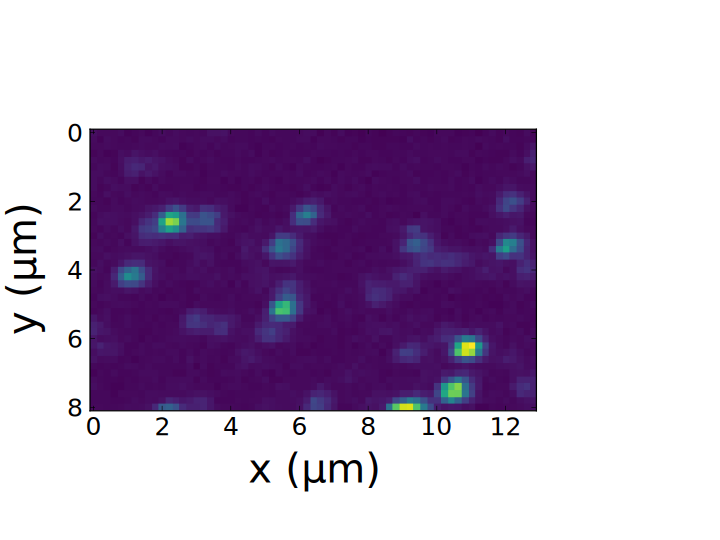
\includegraphics[trim = 0 20 70 50,  clip= true, width = \textwidth]{./pics/scan_xy-32_2APD_mum_noscale.png}}
			\caption{}
			\label{subfig::pp_pl_scan}
		\end{subfigure}
		\caption{ (a) Picture recorded with a commercial high resolution laser scanning microscope. The area shaded in blue represents the \pl scan in image (b). (b) \Pl scan of a \SI{8}{\micro\metre}x\SI{13}{\micro\metre}}
	\end{figure}


	\begin{figure}[tp]
		\begin{subfigure}[t]{ 0.49\linewidth}
			\centering
			\testbox{\includegraphics[trim = 0 0 0 0,  clip= true, width = \textwidth]{./pics/Antenna2_upper_right_150923_01.png}}
			\caption{<caption>}
			\label{subfig::antenna_structures_sem}
		\end{subfigure}
		\hfill
		\begin{subfigure}[t]{ 0.49\linewidth}
			\centering
			\testbox{\includegraphics[trim = 0 0 0 0,  clip= true, width = \textwidth]{./pics/Ir27M_mitte_213_151111_13.jpg}}
			\caption{<caption>}
			\label{subfig::antenna_one_structure_sem}
		\end{subfigure}
		\caption{<caption>}
		\label{fig::<fig>}
	\end{figure}

	\begin{figure}[tp]
		\centering
		\testbox{\includegraphics[trim = 0 0 0 0,  clip= true, width = 0.3\textwidth]{./pics/ccd_f301_emitter7.png}}
		\caption{Image of the sample surface of \SI{100}{nm} wet-milled nanodiamonds spin-coated on an \ir substrate illuminated with diffuse white light. The white bars are the horizontal bars of the cross markers which serve as a coarse orientation on the sample surface, the white dots are nanodiamonds, the big black spot is an artifact.}
		\label{fig::ccd_cross_marker}
	\end{figure}

	% \begin{figure}[tp]
	% 	\begin{subfigure}[t]{ 0.49\linewidth}
	% 		\centering
	% 		\testbox{\includegraphics[trim = 0 0 0 0,  clip= true, width = \textwidth]{./pics/Ir27M_mitte_213_151111_18.jpg}}
	% 		\caption{}
	% 		\label{subfig::nd_before_pick_hr}
	% 	\end{subfigure}
	% 	\hfill
	% 	\begin{subfigure}[t]{ 0.49\linewidth}
	% 		\centering
	% 		\testbox{\includegraphics[trim = 0 0 0 0,  clip= true, width = \textwidth]{./pics/Ir27M_mitte_213_151111_21.png}}
	% 		\caption{}
	% 		\label{subfig::nd_before_pick_no_hr}
	% 	\end{subfigure}
	% 	\caption{caption}
	% \end{figure}

	\begin{figure}[tp]
		\begin{subfigure}[t]{ 0.49\linewidth}
			\centering
			\testbox{\includegraphics[trim = 0 0 0 0,  clip= true, width = \textwidth]{./pics/pick_colored.png}}
			\caption{}
			\label{subfig::pick_antenna_sem}
		\end{subfigure}
		\hfill
		\begin{subfigure}[t]{ 0.49\linewidth}
			\centering
			\testbox{\includegraphics[trim = 0 0 0 0,  clip= true, width = \textwidth]{./pics/Ir27M_mitte_213_151111_26_colored.png}}
			\caption{}
			\label{subfig::transfer_antenna_sem}
		\end{subfigure}
		\caption{}
	\end{figure}

	\subsection{Plasmonic Antennas}

	\cite{Curto2010}
	Optical antennas, acting as converters between propagating and localized fields,provide an effective route to couple photons in and out of nanoscale objects. These antennas are the counterparts of conventional radio andmicrowave antennas and operate in the visible regime (1, 2). Optical antennas have been shown to focus optical fields to subdiffraction- limited volumes (3), enhance the excitation and emission of quantum emitters (4–7), and modify their spectra (8). 
	\\
	A characteristic of antennas is their directed emission and reception. So far, the control of di- rectionality has mainly been pursued by photonic crystal structures (9) and surface-plasmon–based devices (10–12). However, for such structures approaching the nanometer scale diffraction can limit the collimated beaming of light. On the other hand, the interaction of quantum emitters with light is best enhanced with microcavities(13, 14). Compared with these approaches, plasmonic nanoantennas offer a much smaller footprint in an open geometry combining strong subwavelength fields and increased transitionrates, together with the prospect of directionality.
	\\
	\cite{Giessen2010}
	from gold, a metal that can develop charge oscillations in its surface layers when excited by optical radiation. These antennas allow visible radia- tion, which has wavelengths of hundreds of nanometers, to couple into a semiconductor quantum dot only a few nanometers in diam- eter, and also direct the emission
	\\
	Good mode- matched antennas reradiate their energy after excitation within a single cycle of the wave. Molecules or quantum dots take nanoseconds or even longer to reradiate their energy. This time scale corresponds to about 1 million oscillations at optical frequencies, and the emission is in all directions.
	\\
	If an atom, molecule, or quantum dot is placed into the near-field of a metallic nanoantenna (within about 1/50th the wavelength of the emitted radiation), its excited state can radiate photons very efficiently to free space (see the fi g- ure, panel B). The quantum emitters can emit a single photon, which can be exploited in quantum optics. Additionally, the nanoantenna can redirect radiation into a defined solid angle in space and impose a specifi c polarization on it.
	\\
	The demonstration of the Purcell effect, which is the acceleration of the decay of the quantum emitter caused by impedance matching by the antenna to free space, could also enhance the radiative emission over nonradiative losses
	\\
	\cite{Novotny2011}
	The electro- magnetic antenna, originally referred to as an ‘aerial’, is a transducer between electromagnetic waves and electric currents, and generally operates in the radiofrequency regime. In analogy with the electro- magnetic antenna, we define the optical antenna as a device thatconverts freely propagating optical radiation into localized energy, and vice versa1.The spatial extent of a receiver or transducer is commonly much smaller than the wavelength of radiation, λ, and is typically of the order of λ/100.
	\\
	Surface plasmon resonances make optical antennas particularly efficient at selected frequencies. A generic antenna problem is illustrated in Fig. 3. It consists of a transmitter and a receiver, both represented by dipoles p. The antenna is introduced to enhance the transmission efficiency from the transmitter to the receiver. This enhancement can be achieved by increasing the total amount of radiation released by the trans- mitter, for which the antenna efficiency is a useful figure of merit:
	\begin{equation}
		p=p
	\end{equation}
	where P is the total power dissipated by the antenna, Prad is the radiated power and Ploss is the power dissipated through other means,such as by absorption in the antenna. However, the transmission efficiency can also be improved by directing the radiation in the direction of the receiver. The efficiency for this process is repre- sented by the directivity:
	\begin{equation}
		p=p
	\end{equation}
	where the angles θ and ϕ represent the direction of observation and p(θ,ϕ) is the angular power density. The combination of antenna effi- ciency and directivity is referred to as the antenna gain:
	\begin{equation}
		p=p
	\end{equation}
	By reciprocity, we can interchange the fields and sources in Fig. 3 to give p1• E2 = p2 • E1, where E1 (E2 ) is the field of dipole p1 (p2 ) evalu- ated at the location of p2 (p1). A good transmitting antenna is therefore also a good receiving antenna. For a transmitter in the form of a two-state quantum emitter, reciprocity leads to a relationship between the emitter’s excitation rate Γexc and its spontaneous emission rate:
	\begin{equation}
		p=p
	\end{equation}
	Here, the superscript ‘o’ refers to the absence of the antenna and the subscript ‘θ’ indicates the polarization state; that is, the electric field vector points in direction of the θ unit vector. An equivalent equation holds for polarization in the ϕ direction. Interestingly, exci- tation in a direction of high directivity allows the excitation rate to be enhanced more strongly than the radiative rate. Another important antenna parameter is the antenna aperture, which is formally the same as the absorption cross-section sigma. Let us consider a dipole-like receiver with a cross-section σo that is not cou- pled to an antenna. The unit vector in the direction of the absorption dipole axis is denoted as np and the incident field at the location of the receiver is Eo . Once we couple the receiver to an antenna, the field at the receiver increases to E and the cross-section or antenna aperture becomes1
	\begin{equation}
		p=p
	\end{equation}
	Thus, the aperture of an optical antenna scales with the local intensity enhancement factor. Theoretical and experimental stud- ies have shown that intensity enhancements of 104–106are readily achievable14,36,37 and hence, for typical molecules with ‘free-space’ cross-sections of sigmao = 1 nm2 , we find that a layer of molecules spaced 0.1–1 μm apart can absorb all of the incident radiation if each molecule is coupled to an optical antenna. Of course, this estimate ignores the coupling between antennas and therefore has limited validity.


	\subsection{Structure of the Plasmonic Antennas} \label{sec::structure_antenna}

	\begin{figure}[tp]
		\centering
		\testbox{\includegraphics[trim = 0 0 0 0,  clip= true, width = 0.3\textwidth]{./pics/place_colored.png}}
		\caption{<caption>}
		\label{fig::place_antenna_sem}
	\end{figure}

	\begin{figure}[tp]
		\centering
		\testbox{\includegraphics[trim = 120 0 0 0,  clip= true, width = 0.3\textwidth]{./pics/ccd_s1_g3_db_g150_d20_rightone.png}}
		\caption{}
		\label{fig::place_ccd}
	\end{figure}

	\begin{figure}[tp]
		\centering
		\testbox{\includegraphics[trim = 0 0 0 0,  clip= true, width = 0.5\textwidth]{./pics/antenna_fdtd_calculation.png}}
		\caption{<caption>}
		\label{fig::antenna_fdtd_calculation}
	\end{figure}

	FDTD numerical simulations were performed using Lumerical software to characterize gold double bowtie nanoantennas on a gold substrate. The nanoantennas are tailored to have a gap of g = \SI{150}{nm} (taking into account the diameter of the nanodiamonds of around \SI{100}{nm}), side length of L = \SI{2}{\micro\meter}, and a thickness of t = \SI{60}{nm} (see Fig.3a). 
	Upon excitation with incident light, an intense electromagnetic hotspot is formed in the nanoantenna gap \cite{Rahbany2015}\todo{read paper}, which is expected to excite a nanodiamond containing SIV centers aiming to enhance its fluorescence emission. 
	Unlike a single bowtie that is sensitive only to the polarization along its principle axis (C2 rotational symmetry), a double bowtie features a C4 rotational symmetry and therefore focuses both parallel and perpendicular polarizations (i.e. all in-plane directions).
	% For that, a circularly polarized light with a wavelength range of λ = 400 - 1500 nm is chosen to illuminate a gold double bowtie nanoantenna on a gold substrate, which efficiently excites both the horizontal and vertical components of the structure. 
	The index of refraction of gold is taken from Palik \cite{}\todo{Palik, E. D. Handbook of optical constants of solids. 3, (Academic press, 1998)}, and that of the nanodiamond is chosen to be n = 2.4 at $\lambda$ = \SI{660}{nm}. 
	The electric field intensity in the nanoantenna gap is then measured as a function of wavelength to identify the antenna resonance. 
	The spectrum is given in Fig.3b where we observe that the resonance shows two peaks; an intense peak coinciding with the SiV emission wavelength ($\lambda$ = \SI{739}{nm}), and an additional mode at a lower wavelength ($\lambda$ = \SI{710}{nm}) \cite{Rahbany2016}
	The resonance spectrum of the antenna alone shows only one peak at \SI{739}{nm}. 
	Thus, the additional peak is attributed to the presence of the nanodiamond that is slightly shifted from the center of the gap, corresponding to our experimental conditions.
	These calculations suggest, that the emission from an \siv at \SI{738}{nm} is effectively enhanced and directed by the antenna.

	\subsection{\siv in a Plasmonic Double Bowtie Antenna}

		% Einleitung
		In the following, specific details and challenges concerning the coupling process are given and results of the spectroscopic measurements of an \siv in a plasmonic double bowtie antenna are reported.
		\\
		% additional methods
		We performed coupling the nanodiamonds containing \sivs in two approaches:
		First we chose a \nd containing several \sivs for \pp and afterwards a \nd containing a single \siv.
		As mentioned before, single \sivs may be damaged by the electron radiation in the SEM during \pp and stop emittig \pl light.
		Hence, we decided to run first experiments with \nds containing multiple \sivs. 
		This approach has the advantages that we are able to gain experience in the execution of the \pp process without the risk of permanently damaging the emitter and therefore rendering the tedious \pp process futile. 
		For measurements of the intensity enhancement by the antenna, a single emitter is necessary.
		However, the antenna's influence on the \siv spectrum can be studied when serveral emitters are present.
		Therefore, studies of the spectrum are performed in this first approach.
		\\
		After we gained experience with the first approach, we  searched for a suited \nd containing a single \siv.
		The aim was to perform saturation and second order correlation measurements to probe single SiV centers, and consequently quantify the exact Purcell enhancement imposed by the nanoantenna on a single photon emitter.
		% However, the challenges for experiments with a single \siv are magnitudes bigger than for multiple \sivs.



		\subsubsection{\Nd With Multiple \sivs Coupled to Antenna}

			The \nds exploited for the approach of coupling multiple \sivs to an antenna were produced by a wet-milling process from a CVD diamond film\footnote{wet-milling performed by \muzha, diamond film grown by group of \williams} .
			The solution of \nds which exhibit a median size of \SI{100}{nm} were spin-coated on an iridium substrate treated with Piranha etch. 
			To ensure that a pre-characterized nanodiamond exhibiting preferred optical properties (eg. narrow linewidth, high count rate) is later found again, the iridium substrate was engraved with reference cross markers produced by a focused ion beam prior to the spin-coating process.
			After spin-coating, the sample was placed in an oven for 3 hours at \SI{450}{\celsius} to oxidize the surface and remove any residual graphite and amorphous carbon. 
			\\
			% preselection
			% Fig. 1c shows an example of a PL scan where bright spots (highlighted by the red circles) correspond to nanodiamonds with PL in the SiV center spectral range. To further verify the presence of SiV centers, PL spectra at room temperature are recorded.
			\Cref{subfig::spectrum_antenna_nd_multiple} shows the spectrum recorded of the preselected \nd.
			The ZPL peak exhibits a \wl of \SI{738.55\pm0.01}{nm} and a \lw of \SI{5.0\pm0.03}{nm}\todo{fehlergrenzen verfnuenftig machen}.
			These numbers correspond well to the ZPL of unstrained SiV centers and therefore allows us to deduce that the studied nanodiamond contains at least one SiV center.
			Photon autocorrelation measurements revealed, that the \nd contains multiple \sivs.
			\\
			% position
			To determine the position of the \nd on the original substrate, first a scan with a commercial \lsm (LSM) was performed as described in \cref{subsec::position}.
			\Cref{subfig::cross_laser_scan} shows a part of an obtained LSM image.
			The cross marker can easily be identified, the black dots are \nds.
			After transferring the sample into the confocal setup, confocal scans of the corresponding areas are performed (\cref{subfig::pp_pl_scan}).
			The area corresponding to the \fl scan in \cref{subfig::pp_pl_scan} is shaded blue in \cref{subfig::cross_laser_scan}.
			When looking closely, the bright spots in the \fl scan can be identified with \nds visible in \cref{subfig::cross_laser_scan}.
			The image in the SEM is very similar to the image obtained by the LSM.
			Therefore, once a \nd containing a preselected emitter is identified in the LSM scan, it is easy to find the same emitter in the SEM.
			\\
			% A long pass filter (λ = 720 nm) is placed in the detection path to suppress any signal stemming  from the laser.. During the PL scan, the laser spot scans the surface and the emitted PL is recorded by the APD. In front of the APD a 730-750nm bandpass filter is installed. The center wavelength of the zero-phonon line of an SiV center is located at around 738 nm. Therefore, if a nanodiamond contains an SiV center, its emission  will results in a bright spot in the PL scan. 
			% transfer
			The the picking part of the \pp process was performed in the same manner as described in the section about VCSELs (\cref{subsec::vcsel_structure}).
			The gold surface of the plasmonic antenna caused a high adhesion between the antenna surface and the \nd.
			Once the \nd touched the gold, it could not be picked up again with the tungsten tip.
			The \nd first touched the antnna structure a few nanometers away from the gap and immediately sticked to the surface, on top of one of the triangles.
			Therefore, the \nd had to be pushed into the gap with the nanomanipulator tip.
			This process caused some damage to the antenna structure.
			The damage is visible as black area at the tip of the top triangle in \cref{fig::place_antenna_sem}.
			However, FDTD simulations of damaged antennas reveal that this modification of the antenna hardly influences the antenna resonance\todo{bild dazu}.
			\\
			% Spectroscopic measurements
			After this deterministic placement we measure the PL spectrum of the nanodiamond to identify the effect of the nanoantenna on its emission. The result is displayed in \cref{subfig::spectrum_antenna_nd_multiple}.
			% Fig. 7a where an increase in the PL intensity is observed by more than a factor 10 indicating that the nanoantennas indeed contribute to the enhancement of the SiV centers emission. 
			% A $\lambda$ = 710 nm long pass filter is used to eliminate any signal from the laser. 
			The additional peak at a lower wavelength is attributed to the antenna resonance mode. 
			To verify this, we convolute the experimental PL spectrum of the nanodiamond measured before placing it in the nanoantenna (\cref{subfig::spectrum_nd_multiple}) with the intensity spectrum of the nanoantenna obtained by simulations (\cref{fig::antenna_fdtd_calculation}). 
			The resulting spectrum is given in \cref{subfig::antenna_convolution}, and is in good agreement with the measured spectrum in \cref{subfig::spectrum_antenna_nd_multiple}, confirming that indeed the extra peak is due to the antenna resonance.

			\begin{figure}[tp]
				\begin{subfigure}[t]{ 0.49\linewidth}
					\centering
					\testbox{\includegraphics[trim = 0 0 0 0,  clip= true, width = \textwidth]{./pics/xy_scan-11_2APD.png}}
					\caption{}
					\label{subfig::antenna_laser_scan}
				\end{subfigure}
				\hfill
				\begin{subfigure}[t]{ 0.49\linewidth}
					\centering
					\testbox{\includegraphics[trim = 0 0 0 0,  clip= true, width = \textwidth]{./pics/xy_scan-13_2APD.png}}
					\caption{
					}
					\label{subfig::antenna_bowtie_laser_scan}
				\end{subfigure}
				\caption{<caption>}
			\end{figure}

			% \begin{figure}[tp]
			% 	\centering
			% 	\testbox{\includegraphics[trim = 0 0 0 0,  clip= true, width = 0.3\textwidth]{./pics/antenna_no_ND.pdf}}
			% 	\caption{<caption>}
			% 	\label{fig::spectrum_antenna_multiple_before}
			% \end{figure}

			\begin{figure}[tp]
				\begin{subfigure}[t]{ 0.49\linewidth}
					\centering
					\testbox{\includegraphics[trim = 0 0 0 0,  clip= true, width = \textwidth]{./pics/antenna_no_ND.pdf}}
					\caption{}
					\label{subfig::spectrum_antenna_no_nd}
				\end{subfigure}
				\hfill
				\begin{subfigure}[t]{ 0.49\linewidth}
					\centering
					\testbox{\includegraphics[trim = 0 0 0 0,  clip= true, width = \textwidth]{./pics/spe_Ir27M_f200_xy04x13y88_D09_t30_highP_fit.pdf}}
					\caption{}
					\label{subfig::spectrum_nd_multiple}
				\end{subfigure}
				\caption{<caption>}
			\end{figure}

			\begin{figure}[tp]
				\begin{subfigure}[t]{ 0.49\linewidth}
					\centering
					\testbox{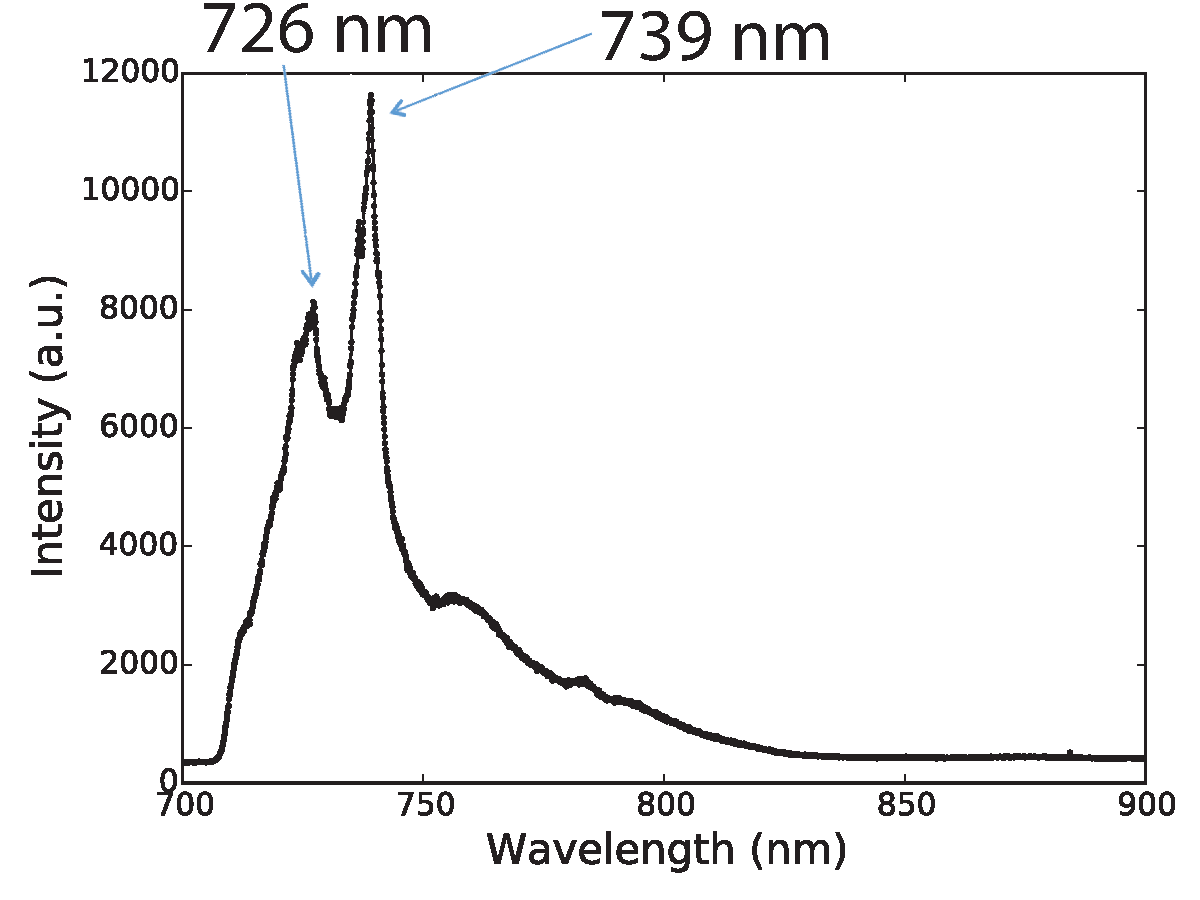
\includegraphics[trim = 0 0 0 0,  clip= true, width = \textwidth]{./pics/find_middle_with_ccd_highP_2_arrows.pdf}}
					\caption{}
					\label{subfig::spectrum_antenna_nd_multiple}
				\end{subfigure}
				\hfill
				\begin{subfigure}[t]{ 0.49\linewidth}
					\centering
					\testbox{\includegraphics[trim = 0 0 0 0,  clip= true, width = \textwidth]{./pics/antenna_convolution.png}}
					\caption{}
					\label{subfig::antenna_convolution}
				\end{subfigure}
				\caption{<caption>}
			\end{figure}

		\subsubsection{\Nd With Single \siv Coupled to Antenna}
			sample M02-16: drop-casted with SiGH45
			% preselection, 
			First, only a small percentage of the technically suited \nds (size, isolation) contain a single \siv, second, damage due to electon radiation during \pp.
			After  an \siv with a small dig in the \gt function, indicating only few \sivs.
			% position
			% transfer
			% Spectroscopic measurements

			\begin{figure}[tp]
				\begin{subfigure}[t]{ 0.49\linewidth}
					\centering
					\testbox{\includegraphics[trim = 0 0 0 0,  clip= true, width = \textwidth]{./pics/sat114_fit_bkg.pdf}}
					\caption{}
					\label{subfig::single_siv_sat_before_transfer_antenna}
				\end{subfigure}
				\hfill
				\begin{subfigure}[t]{ 0.49\linewidth}
					\centering
					\testbox{\includegraphics[trim = 0 0 0 0,  clip= true, width = \textwidth]{./pics/g2_sat113_5mW_corr_fit.pdf}}
					\caption{}
					\label{subfig::single_siv_g2_before_transfer_antenna}
				\end{subfigure}
				\caption{<caption>}
			\end{figure}

			\begin{figure}[tp]
				\begin{subfigure}[t]{ 0.49\linewidth}
					\centering
					\testbox{\includegraphics[trim = 0 0 0 0,  clip= true, width = \textwidth]{./pics/single_spectrum_sat113_fit.pdf}}
					\caption{}
					\label{subfig::single_siv_spec_before_transfer_antenna}
				\end{subfigure}
				\hfill
				\begin{subfigure}[t]{ 0.49\linewidth}
					\centering
					\testbox{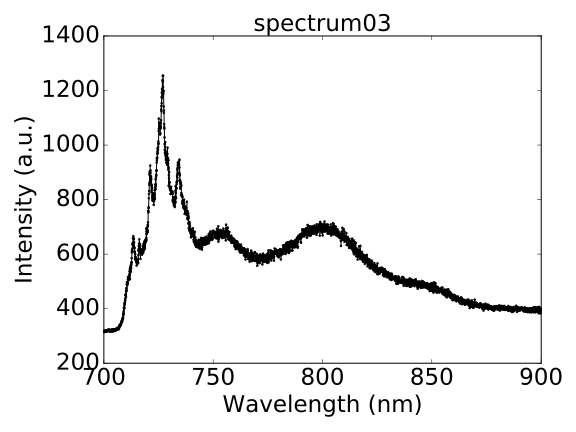
\includegraphics[trim = 0 0 0 0,  clip= true, width = \textwidth]{./pics/spectrum03.pdf}}
					\caption{}
					\label{subfig::single_siv_spec_after_transfer_antenna}
				\end{subfigure}
				\caption{<caption>}
			\end{figure}

			\begin{figure}[tp]
				\begin{subfigure}[t]{ 0.49\linewidth}
					\centering
					\testbox{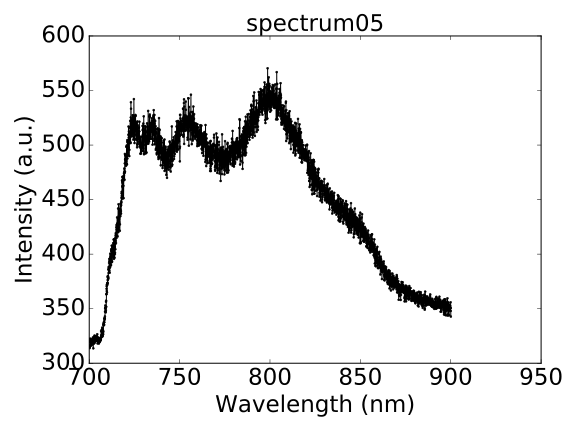
\includegraphics[trim = 0 0 0 0,  clip= true, width = \textwidth]{./pics/spectrum05.pdf}}
					\caption{}
					\label{subfig::single_siv_spec_bkg_antenna}
				\end{subfigure}
				\hfill
				\begin{subfigure}[t]{ 0.49\linewidth}
					\centering
					\testbox{\includegraphics[trim = 0 0 0 0,  clip= true, width = \textwidth]{./pics/spectrum_sat113_fit_origin.pdf}}
					\caption{}
					\label{subfig::single_siv_spec_after_transfer_antenna_bkg_corrected}
				\end{subfigure}
				\caption{<caption>}
			\end{figure}
